\documentclass[10pt,letterpaper]{article}
\usepackage{enumitem}
\usepackage[utf8]{inputenc}
\usepackage[spanish]{babel}
\usepackage{graphicx}
\usepackage{amsmath}
\usepackage{amsfonts}
\usepackage{amssymb}
\usepackage{makeidx}
\usepackage{graphicx}
\usepackage{url}
\usepackage{hyperref}
\usepackage{minted}
\usepackage[dvipsnames]{xcolor}
\usepackage[left=2cm,right=2cm,top=1.5cm,bottom=1.5cm]{geometry}
\usepackage{biblatex}
\addbibresource{Bib.bib}

\begin{document}

\thispagestyle{empty}
	
	\begin{figure}[ht]
	   \minipage{0.76\textwidth}
			\includegraphics[width=4cm]{Proyecto/IMAGES/Logo_UNAM.png}
			\label{EscudoUNAM}
	   \endminipage
	   \minipage{0.32\textwidth}
			\includegraphics[height = 4.9cm ,width=4cm]{Proyecto/IMAGES/Logo_FC.png}
			\label{EscudoFC}
		\endminipage
	\end{figure}
	
	\begin{center}
	\vspace{0.8cm}
	\LARGE
	UNIVERSIDAD NACIONAL AUTÓNOMA DE MÉXICO 
	
	\vspace{0.8cm}
	\LARGE
	FACULTAD DE CIENCIAS
	
	\vspace{.5cm}	
	\Large
	\textbf{Práctica 3}

	\vspace{.7cm}
	\normalsize	
	EQUIPO \\
	\vspace{.3cm}
	\large
	\textbf{Arroyo Martínez Erick Daniel} \\ 
    \textbf{Terrazas Rivera Alex}\\
    \textbf{Vergara Navarro Mixtli Arturo}
	\vspace{.7cm}\\
	\normalsize	
	PROFESOR \\
	\vspace{.3cm}
	\large
	\textbf{Gilde Valeria Rodríguez Jiménez}

    \vspace{.7cm}
	\normalsize	
	AYUDANTES \\
	\vspace{.3cm}
	\large
	\textbf{Rogelio Alcantar Arenas}\\
    \textbf{Gibran Aguilar Zuñiga}\\
    \textbf{Luis Angel Leyva Castillo}\\
    \textbf{Rogelio Alcantar Arenas}
	
	\vspace{.7cm}
	\normalsize	
	ASIGNATURA \\
	\vspace{.3cm}
	\large
	\textbf{Computación Concurrente}
	
	\vspace{.2cm}
	\today
	\end{center}
	\newpage

%%% Indice
%\tableofcontents
%\newpage
\section*{Introducción}
Este trabajo consiste en resolver una versión del problema de los cien prisioneros, los ajustes de está versión son que se trabaja con un número arbitrario de prisioneros y con un estado inicial pseudoaleatorio del interruptor. La estategia seguida para resolver el problema es similar a la utilizada para resolver el problema origina, es decir, designarle la responsabilidad de decidir a un solo prisionero (Vocero), este tendrá como condición de parada contar hasta \textbf{2n-2} cambios de estados en el interruptor.

\section*{Cuestionario}

Tu solución propuesta cumple:

\begin{itemize}
    \item Exclusión Mutua:
    Nuestra primer impresión es que nuestra implementación podría no garantizar cumplir esta propiedad. Pues podrían existir estados del sistema que permitan que más de un hilo entre a la sección crítica. Sin embargo, si asumimos que el el rentrantlock puede garantizar la exclusión mutua entonces esto implicaría que el sistema cumple la misma propiedad. A grandes rasgos en nuestra implementación, cuando se lanzan todos lo hilos, estos comienzan el sorteo para obtener el lock, una vez que un hilo toma el lock, este mismo, bloquea los demás hilos hasta que el que ingreso libere el mismo candado (es decir que salga de las sección crítica).

    \item No Deadlock:
    Por la definición de deadlock,tenemos que este caso ocurre cuando, al menos, dos hilos quedan bloqueados por un recurso que otro hilo, en las mismas circunstancias, debe liberar una vez que acceda a otro recurso bloqueado. En este caso, dado que nuestro hilo cumple exclusión mutua, es decir, que solo puede entrar un hilo a la vez. Además, dada la implementación de nuestra sección crítica, el hilo que entre, liberara en algún momento  la sección crítica sin mayor problema, pues no hay dependencias a otros recursos. Por lo tanto, si garantizamos que todo hilo que entre a la sección crítica (que ganó el lock) saldrá. Entonces, nuestro sistema cumple con NO deadlock.

    \item Libre de Hambruna:
    Tras revisar algunos escenarios de ejecución de nuestra implementación, tenemos que, existen algunos escenarios en los que un hilo queda bloqueado por más tiempo que cualquier otro. Lo que implica que, al menos, un hilo no puede acceder a la sección crítica. Esto implicaría la intrusión de hambruna en el sistema, pues en nuestras simulaciones la ejecución se extiende de forma indeterminada. Adicional a la indeterminación que los sistemas concurrentes asumen, al conseguir un escenario en el que un hilo no puede acceder a la sección crítica. Entonces, no podemos garantizar que nuestra implementación, en particular, el uso de Thread.sleep(500) en el método run podría afectar la justicia del sistema, y disminuir así la persistencia de NO hambruna en el sistema, pues ya que un hilo que ha salido de la sección crítica podría tener que esperar antes de volver a entrar y este punto generar el escenario adecuado para que este hilo no termine su tarea, y por tanto, no termine nuestra ejecución.
\end{itemize}

De ser así, demuestra cada propiedad.


\hspace{3mm}

Además contesta las siguientes preguntas justificando lo siguiente

\begin{itemize}
    \item ¿Tu solución cumple para n prisioneros?

    Sí se cumple para $n$ prisioneros, siempre y cuando no se encuentre con condiciones de carrera ya que cada prisionero se asegurará de prender el interruptor dos veces y el vocero contará que el interruptor haya sido prendido $2(n - 1)$ si el interruptor empieza en false simplemente contará a todos dos veces exactas y si el interruptor empieza en true, cómo el vocero no puede saber si lo puso en ese estado un prisionero o si empezó en ese estado, entonces, el vocero asumirá que lo puso en ese estado el prisionero y habrá contado uno de más y, por lo tanto, contará a $2 (n-2)$ prisioneros dos veces y a un prisionero lo contará una sola vez, lo que significa que cuando mande el mensaje de que todos acabaron podremos estar seguros de que todos ya pasaron por lo menos una vez.

    \item Si tu programa tarda mucho en terminar, ¿por que crees que pasa esto? 

    Cuando un prisionero prende el interruptor todo prisionero que no sea el vocero y entre después de él no hará nada hasta que el vocero vuelva a apagar el interruptor, por lo tanto va a haber muchas veces en las que entre un prisionero a una habitación y no suceda nada y simplemente se gasta el tiempo del procesador.

    \item De la pregunta anterior, que podrías proponer para mejorar los tiempos.

    Podríamos darle una prioridad mayor al vocero para que pase más veces a la habitación que el prisionero normal y si ya pasó un prisionero tal vez se le pueda bajar la prioridad, esto nos ayudaría a que no haya tantos prisioneros entre el que prende el interruptor y el vocero que la apaga, lo que significa que ya no tendríamos tantos tiempos muertos.
\end{itemize}

Estas preguntas debes contestarlas para cada versión del problema (en caso de que realices ambos).

\hspace{3mm}

Por ultimo, analiza bien el siguiente enunciado:
“Si los candados cumplen con exclusión mutua, no deadlock o libre de hambruna, es decir, con las propiedades para un candado seguro, entonces el sistema donde lo utilizamos también las cumplirá.”

De esto justifica porque si se cumple o porque no.

No necesariamente se cumple ya que importa de igual manera tanto la implementación del candado cómo su ubicación en el código lo que implica que cuando se implemente en el sistema se deberá identificar correctamente todas las secciones críticas ya que si no se hace esto no se pueden garantizar todas las propiedades para todo el sistema.


\hspace{3mm}

Añade lo aprendido en esta practica, así como las dificultades que tuviste para realizarla.

En esta práctica logramos implementar una solución para el problema de los prisioneros modificado, la solución que se implemento fue casi la misma del problema original pero en vez de que el vocero contará a cada prisionero una sola vez lo modificamos para que contara a cada uno dos veces lo cual provoca que, independientemente empiece el interruptor prendido o apagado, el vocero siempre contará a todos los prisioneros por lo menos una vez.

La única dificultad que nos encontramos fueron unas condiciones de carrera dónde dos o más prisioneros prenden el interruptor al mismo tiempo provocando que el vocero nunca llegue al conteo final, esto se puede solucionar fácilmente al sincronizar la función dónde entran a la habitación

%% Desarrollo
%% Referencias
\section*{Diagrama UML}
\begin{figure}[H]
    \centering
    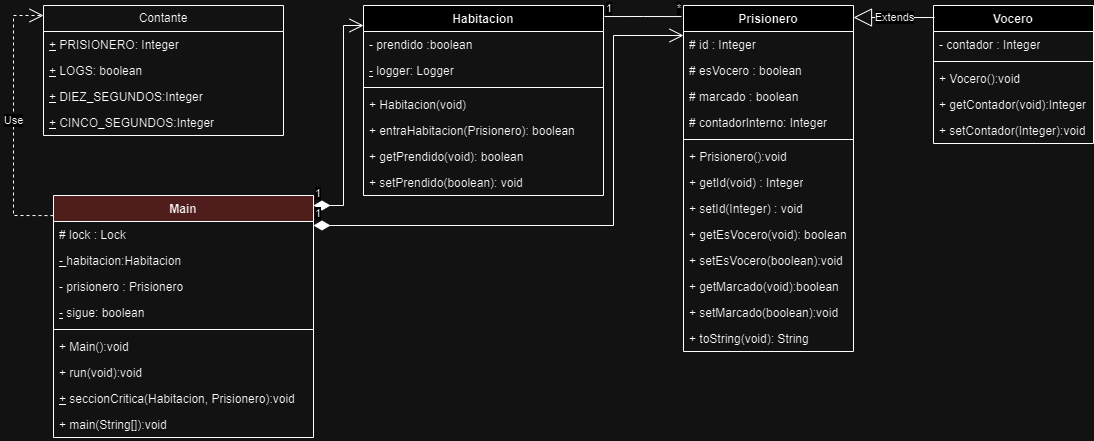
\includegraphics[width=0.7\linewidth]{P03//IMG/diagrama_P3.png}
    \caption{Enter Caption}
    \label{fig:enter-label}
\end{figure}
\section*{Referencias}
\begin{itemize}
    \item Gafni, E. (2018) Group mutual exclusion in linear time and space. Recuperado de: \url{https://www.sciencedirect.com/science/article/pii/S0304397517304747}
\end{itemize}
%\printbibliography[heading=bibintoc, title={Referencias bibliográficas} ]
\end{document}